%\documentclass[12pt]{article}
%\usepackage[a4paper, margin=1in]{geometry} 
%\usepackage{graphicx} 
%\usepackage{hyperref}
%\usepackage{float}
%\usepackage{multicol}
%\usepackage[font=small, labelfont=bf]{caption}
%
%\begin{document}

%
% Alignment by brute-force
%
\subsection{Table representation of alignment}
Several data structures can be used to represent an alignment. The table representation is frequently used and also makes the process clear when we combine it with dynamic programming (DP) later.

\subsubsection*{Data structures and algorithms}
It is important to consider the following aspects before solving computational problems.
\begin{enumerate}
\item Identify and analyze the problem you want to solve
\item Pick up an algorithm that can efficiently solve the problem
\item Decide a data structure that works with the algorithm of your choice
\end{enumerate}

\noindent We use a table format (2D array) to solve global alignments by dynamic programming.

\subsubsection*{Example of table format}
Alignment:
\begin{verbatim}
    q: -AG-
    d: A-CG
\end{verbatim}
\medskip 

\noindent \textbf{1. Initial setup}

\begin{enumerate}
\item Make a table with the size of (1 + length(q)) by (1 + length(d))
\item Add the database sequence as column labels
\item And the query sequence as row labels
\end{enumerate}

\begin{figure}[H]
  \centering
      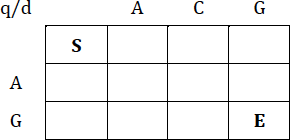
\includegraphics[width=0.3\textwidth]{fig02/alignment_to_table.png}
\end{figure}

\noindent \textbf{2. Add arrows}

We use three types of arrows to form an alignment.
\begin{itemize}
\item Move diagonally: add the letters from ‘q’ and ‘d’ to the alignment
\item Move vertically: add ‘-’ and the letter from ‘d’ to the alignment
\item Move horizontally: add the letter from ‘q’ and ‘-’ to the alignment
\end{itemize}

It should start from S and stops at E.

\begin{figure}[H]
  \centering
      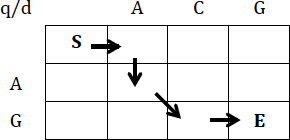
\includegraphics[width=0.3\textwidth]{fig02/alignment_to_table_example.png}
\end{figure}

%
% Exercise \thesection.3
%
\subsubsection*{Exercise \thesection.3}

Find the corresponding alignments for Table 1, 2 and 3.

\begin{multicols}{3}
Table 1
\begin{figure}[H]
  \centering
      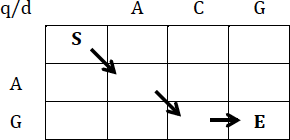
\includegraphics[width=0.3\textwidth]{fig02/alignment_to_table_exercise_1.png}
\end{figure}

Table 2
\begin{figure}[H]
  \centering
      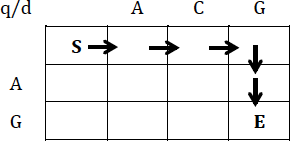
\includegraphics[width=0.3\textwidth]{fig02/alignment_to_table_exercise_2.png}
\end{figure}

Table 3
\begin{figure}[H]
  \centering
      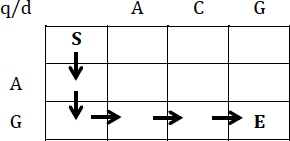
\includegraphics[width=0.3\textwidth]{fig02/alignment_to_table_exercise_3.png}
\end{figure}

\end{multicols} 

%\end{document}
